\section{Phase 1: Online Survey}

\begin{figure}
	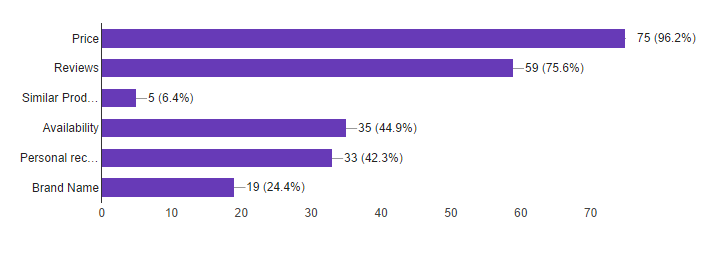
\includegraphics[width=0.9\columnwidth]{figures/ShoppingFactors}
	\caption{Most important factors in making shopping decisions}
	\label{figures:ShoppingFactors}
\end{figure}

 \subsection{Methodology}
We distributed a preliminary survey over social media to identify important aspects of customers' in-store and online shopping experiences and received responses from 78 participants. We asked participants to identify the three most important pieces of information involved their shopping decisions, what they did and did not like about existing in-store and online shopping experiences, and ways they currently use technology in shopping. \todo{does this feel like a reasonable synopsis?}  \todo{JRB: Yes, except I would like to know if these were open-ended questions or not.}
We used the responses from our online survey to
%isolate -- JRB: WC?
identify 
factors of in-store and online shopping that were most important to our participants.  Relevant to the current paper, we asked participants if they use a mobile device while in-store to make purchasing decisions, and to select important factors from a list we provided. Figure \ref{figures:ShoppingFactors} details participants' responses when prompted for their three most important factors in making shopping decisions. Using open-ended questions, we asked participants what they liked the most and least about shopping online and in store. We clustered responses based on similarity, resulting in the findings below.

%% JRB -- Removed, not needed: \subsection{Findings}
Participants appreciate the immediacy and physical interaction with products in a store, but cited drawbacks included the inability to comparison shop, to get the lowest price and/or feeling that they are paying too much, and store staff trying to influence purchase decisions.  Participants appreciate the freedom from store location and hours, \todo{I'm not sure what "freedom from store location and hours" means - EH} \todo{JRB: Ditto.} and time-to-completion of online shopping, \todo{I'm confused as to whether you're talking about things participants appreciate about in-store shopping or about online shopping} but said they dislike the shipping charges and wait times associate with online shopping. We also found that users are willing to spend more time researching more expensive products. These findings provided a foundation from which we engage in our design work in phases 2 and 3.
